\documentclass[a4paper,10pt,twoside]{article}

% Note that if you want to use the \begin{equation} ... \end{equation}
% environment, you will have to include fleqn in the
% \documentclass[...]{...} options! 
% The top of your LaTeX file should then look like this:
% \documentclass[a4paper,10pt,twoside,fleqn]{article}

\usepackage{clin}        % Stylefile for CLIN Journal
\usepackage{harvard}     % Bibliography Stylefile
%\usepackage{...,cgloss4e,avm,trees,tree-dvips,gb4e,ipa,graphicx}
                         % Whatever other packages you need
% Harvard:
% \cite{Covington}             (Covington 1994)
% \citeasnoun{Covington}       Covington (1994)
% \citeyear{Covington}         (1994)


%tikz packages for drawing grammar trees
\usepackage{tikz}
\usepackage{tikz-qtree}
\usetikzlibrary{positioning}

\usepackage{amsmath,amssymb}

\pagestyle{empty}

\begin{document}

\title{Neural processing of sentences}

%Authors and addresses
%Example has 3 authors with 2 different affiliations
%Adapt where necessary
\author{Amelia Burroughs$^*$ \email{amelia.burroughs@bristol.ac.uk}\\
{\normalsize \bf Nina Kazanina}$^{**}$ \email{nina.kazanina@bristol.ac.uk}\\
{\normalsize \bf Conor Houghton}$^*$ \email{conor.houghton@bristol.ac.uk}
\AND \addr{$^*$Department of Computer Science, University of Bristol, UK}
\AND \addr{$^{**}$School of Psychological Science, University of Bristol, UK} }


\maketitle\thispagestyle{empty} % extra pagestyle command for first page

\begin{abstract}

How the human cognitive system is able to comprehend language has been
a matter of recent debate. 
%
%
On the one hand the brain may make use of
learned grammatical rules to decompose sentences into a hierarchy of
syntactic structures to generate meaning. On the other hand the brain
may rely on simpler, statistical methods where the generation of
meaning relies on sequential processing. 
%
%
Cortical activity has been
shown to track speech at the rate of syllable, phrase and sentence
presentation. 
%
%
Our goal
is to shed light on the extent to which hierarchical structure plays a role in language processing during sentence comprehension as measured by the cortical tracking of phrases. To this end we use human EEG to record from participants as they listen to streams of four word sentences. 
%
%
We confirm that cortical activity does synchronise with the rate at which syllables, phrases and sentences
are presented. 
%
%
Sentence stimuli that contain both appropriate grammar
and semantic information generate a full brain response at the rate of
phrase presentation. This response is reduced if either grammar or
semantic information is absent. In sentences that lack both correct
grammar and meaningful semantics, the response at the phrasal rate
disappears. 
%
%
This suggests that both syntax and semantics are important
contributors during sentence processing, as opposed to just syntax
alone. 
%

\end{abstract}

\section{Introduction}

The ability of the human brain to rapidly generate meaning from an
incoming stream of sentences during natural language is
impressive. There are two competing, but not necessarily exclusive, theories describing how we are able to process words. Both of these theories suggest that the smaller discrete units of language,
such as words and phrases, are concatenated by the brain into larger
units, such as sentences. What is under debate is the principles that
govern this organisation: one theory argues for the primacy of a
learned rule-based grammar, the other, for the primacy of statistical
relationships between the discrete units.

In natural language the majority of utterances are composed of several
words that are put together in a sequence according to a set of
predefined rules that determine the serial order of language
elements. It is therefore of interest to understand how the brain
realises these rules. Linguists typically describe sentences in terms
of a hierarchical syntactic structure with a tree-like hierarchy of
nested phrases.

In support of this point-of-view, it has been demonstrated, using MEG
in \cite{DingEtAl2016} and using EEG in \cite{DingEtAl2017} that
cortical activity can entrain to the rate of syllable, phrase and
sentence presentation. In the EEG experiments participants were played
continuous streams of four-word sentences, where each word was 320 ms
long in duration and consisted of only a single syllable. As in
Fig.~\ref{fig:freq_tree} each sentence was composed of a noun phrase
and a verb phrase, which both contained two words. Thus these stimuli
have a specific frequency at three levels of linguistic structure:
syllables at 4/1.28 Hz, phrases at 2/1.28 Hz and sentences at 1/1.28
Hz. The neural responses were analysed using time-frequency
decomposition and measures of inter-trial phase coherence
(ITPC). Cortical activity was found to be phase-locked to the rate of
presentation of syllables, phrases and sentences even though only the
syllable frequency is present in the auditory signal itself, the other two
frequencies rely on the meaning of the words and the structure of the
sentences.  This can be interpreted as evidence for neural
entrainment to discrete higher-level syntactic structures, as opposed
to neural tracking of, for example, transition probabilities during
sentence processing.

\begin{figure}[tb]
\begin{center}
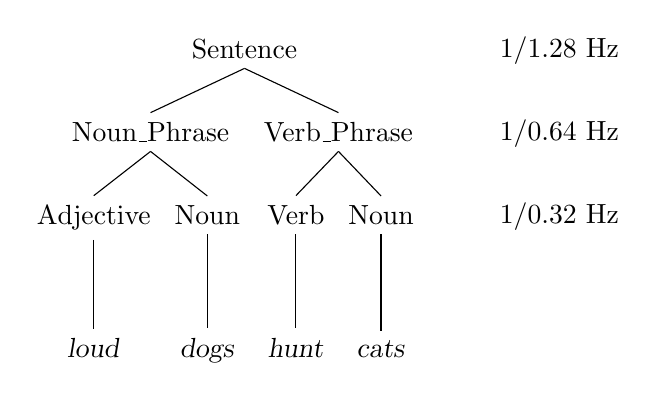
\begin{tikzpicture}
\tikzset{every tree node/.style={align=center,anchor=base}}
\tikzset{level 5+/.style={level distance=2\baselineskip}}
\tikzset{frontier/.style={distance from root=9\baselineskip}}
\Tree
    [.Sentence     
      [.Noun\_Phrase
        [.Adjective {\textsl{loud}} ]
        [.Noun  {\textsl{dogs}} ]
      ]
      [.Verb\_Phrase 
        [.Verb {\textsl{hunt}} ]
        [.Noun {\textsl{cats}} ]
      ]
    ]
 \node at (4,0.1) {1/1.28 Hz};
 \node at (4,-0.95) {1/0.64 Hz};
 \node at (4,-2.0) {1/0.32 Hz};
\end{tikzpicture}
\end{center}
\caption{Tree with frequencies \label{fig:freq_tree}}
\end{figure}

However, a considerable amount of behavioural data highlights the
significance of statistics during language comprehension. At the level
of word-statistics, word recognition times can largely be determined
by their frequency of occurrence in the language, word reading times
have been found to closely correlate with word probability and when an
ambiguous sentence has to be interpreted, the most probable
interpretation is most likely to be chosen (for review see
\cite{Jurafsky2002}). Additionally, both reading times and the
amplitude of neural responses are graded by the strength of
constraints imposed by prior context on possible sentence
continuations \cite{GibsonPearlmutter1998}. Language statistics must
therefore play a role in human language processing. 

In a statistical description, the brain, in a
Bayesian manner, exploits the rich statistical structure of language
to predict possible identities for syllables, words and phrases and
uses these predictions to aid the identification of the actual
linguistic input. In this picture, the interpretation of language
involves the production, reevaluation and resolution of predictions,
and grammar has evolved out of a kind of \lq{}language game\rq{} where
speakers aid each other by propagating conventions about how words are
arranged, enriching the statistical structure of utterances and syntactic categories are not psychologically real, but epiphenomenal to a statistical-based response to linguistic
stimuli.

In this context \cite{FrankYang2018} propose a computational model that
assumes no higher level of abstraction than a semantic
clustering of word representations. Their model represents each word
as a high-dimensional vector chosen so that the proximity structure of
the vectors matches the statistical relationship between the
corresponding words in a large language corpus. The frequency tagged
experiment from \cite{DingEtAl2016}, described above, were simulated
and the model generated power peaks at the same frequencies as those
observed experimentally. This suggests that the peaks could be
generated using only the lexical information within the word stimuli,
without the need for any knowledge of syntax. 

Here human electroencephalography (EEG) is used to measure responses to
simple meaningful sentences in comparison to sentences with two different
manipulations; nonsense sentences which have been deliberately chosen
to have little sensible meaning, and re-ordered sentences, in which
syntax has been destroyed by re-ordering the words. The aim of this
experiment is to help to distinguish between the two competing
explanations for the phrase- and sentence-level phase locking observed
in \cite{DingEtAl2016,DingEtAl2017}.

We used EEG to record neural activity while subjects listened to continuous streams of four single-syllable words that can combine to form a sentence consisting of a noun phrase and a verb phrase. We found that cortical responses become phase-locked to the frequencies at which syllables, phrases and
sentences are presented. A peak in the ITPC value is observed at the sentential rate (1/1.28 Hz). This is similar for sentences that are both grammatically correct and with semantically sensible words and sentences that are ungrammatical in terms of word order and contain semantically
 unrelated words. The peak in the ITPC value at the rate of phrase presentation
 (2/1.28 Hz) is maximal when sentences are both grammatical and make
 semantic sense. This peak is reduced when either grammar or
 semantic sense alone is lacking and is absent when sentences are both ungrammatical and
 lack semantically-related words. 


\section*{Methods}
\subsection*{Participants}

Eighteen right-handed, native English speakers (11 female, mean age 26
years (range 22 - 32 years)) participated in this study. All
participants gave written, informed consent prior to undertaking the
study and were paid £20. Ethical approval for our experimental procedures were obtained from the University of Bristol Faculty of Science ethics board. All methods were performed in accordance with the relevant guidelines and regulations.

\subsection*{Stimuli}

The experimental procedures were similar to those used in a recent EEG
study \cite{DingEtAl2017}. Listeners were played English sentences
composed of four single-syllable words. Each word was synthesised
independently using the MacinTalk Synthesizer (male voice Alex, in Mac
OS X 10.7.5). All of the synthesised words (226 - 365 ms) were
adjusted to 320 ms duration and volume normalised using the freely
available Praat software \cite{BoersmaWeenink2018}.

20 single-syllable words were chosen for each of the four word
categories: adjective, subject, verb, object. Words were selected if
they were synthesised clearly by the speech synthesizer and if they
could be easily categorised into a distinct word category.  This was
to avoid verbs, such as ``ride'' which can
often be used as nouns. Nouns were pluralised and all sentences were
played in the present tense.

Sentences were made by randomly selecting words from each of the four
word categories in the order 
\begin{center}
adjective, subject noun, verb, object noun
\end{center}
These sentences were then independently ranked in terms of how
much sense they made by 290 online participants recruited through
Prolific Academic. Participants were presented with 110 pairs of
sentences, ten of these were an attention trap; participant were asked
to press \lq{F}\rq{} in response to sentences containing the word
\lq{}fish\rq{} and were punished with a time out if they made a
mistake. For the remaining 100 pairs they selected the sentence which
\lq{}sounds more normal in everyday speech\rq{}. Elo
chess ranking \cite{Elo1978} was used to derive individual scores for
each sentence from the pairwise comparisons. This established a
ranking from sense to nonsense. The top 20 sentences were chosen to form the
\lq{}sensical\rq{} sentence conditions and the bottom 20 were chosen to form the \lq{}nonsensical\rq{}
sentence conditions. 

Based on these sensical and nonsensical sentences four different conditions were created: the
original sensical sentences and nonsensical sentences along with two ungrammatical conditions in which the words for sensical and nonsensical sentences were re-ordered as
\begin{center}
     verb, subject noun, object noun, adjective
\end{center}
These four conditions are summarized in Table~\ref{tab:conditions}.

\begin{table}
\begin{tabular}{l|ll}
&sensible&nonsense\\
\hline\\
grammatical&\textbf{GS}: huge trams scare boys&\textbf{GN}: bored mugs write beds\\
ungrammatical &\textbf{US}: scare trams boys huge&\textbf{UN}: write mugs beds bored
\end{tabular}
\caption{A summary of the four conditions; the condition label used in the text is in
  bold, the sentence beside this gives an
  example.\label{tab:conditions}}
\end{table}

\subsection*{Experimental Procedures}

In total, 18 participants listened to 120 trials. For each of the four
conditions, 30 trials were presented. A trial was made up of thirteen
four-word sentences, played back to back in a continuous stream with
no acoustic gap between the sentences. Five trials were put together
to make a block. Each block consisted of five trials of the same
condition with an 800 ms break between trials. At the end of each
block participants were asked to rate the sentences on a scale of one
to five in terms of how much sense the sentences made to them on
average using a button press. Following the button press, the next
block was played after a delay of 1200 ms. Blocks were presented in a
random order and the order of the blocks was counterbalanced across
participants.

\subsection*{EEG Recording}

EEG was continuously recorded with a 32-channel EEG system fitted on a
standard electrode layour elasticised cap using a BrainAmp DC
amplifier (Brain Products GmbH). Signals were digitized at a sampling
rate of 1,000 Hz (bandpass filter = 0.01–400 Hz) and referenced to the
vertex (Cz), as in \cite{DingEtAl2017}. The impedance of the
electrodes was kept below 5kohms. Eyeblink artifacts were removed
using ICA: an independent component was removed if in its topography
the mean power over the most frontal three channels was more than
twenty times stronger than the mean power over all other channels. The
signals of interest are in the low-frequency region, at 1/1.28,
2/1.28, and 4/1.28 Hz and so the EEG signal was lowpass filtered to 25
Hz. Data were referenced offline to a common average reference and the
responses to each individual trial were epoched.

\subsection*{Data analysis}

Upon sound onset there is a transient EEG response and so the first
sentence in each trial was removed from the data. This meant that the
overall trial length was 15.36 seconds (1.28 seconds x 12
sentences). The remaining EEG signal was converted into the frequency
domain using the discrete fourier transform with a frequency
resolution of 0.065 Hz, that is, 1/15.36 Hz. The complex-valued
Fourier coefficient of the trail $k$, $X_k(f)$, is then used to
calculate the inter-trial phase coherence .

The inter-trial phase coherence is defined as
\begin{equation}
\label{eq:itpc}
R(f)=\frac{1}{K}\left[\left(\sum_k{\cos{\theta_k(f)}}\right)^2+\left(\sum_k{\sin{\theta_k(f)}}\right)^2\right]
\end{equation}
where $\theta_k(f)$ is the phase angle of each complex-valued Fourier
coefficient $X_k(f)$ and $K$ is the total number of trials. As with
the evoked power, it measures the time-locked response; because it
uses only the phase-angle rather than the whole response, it does not
show the same $1/f$ noise that is present in the evoked power. As
such, it is a convenient measure of EEG response to a stimulus with
fixed frequency.

As in \cite{DingEtAl2016} a one-tailed paired t-test was used to test
whether the inter-trial phase coherence value in a given frequency bin
was significantly stronger than the average of the neighboring four
frequency bins, two bins on either side. This was applied to all
frequency bins below 5 Hz and a FDR correction for multiple
comparisons was applied.

A repeated measures, two-way ANOVA with a two (grammar: grammatical or
ungrammatical) by two (sense: sensical or nonsensical) factorial
design was performed to compare the main effects of grammar and
sensible meaning on the strength of the ITPC at target frequencies
across conditions. The TukeyHSD post-hoc test was used to compare the
strength of the ITPC responses at different frequencies of interest
(1/1.28 Hz, 2/1.28 Hz and 4/1.28 Hz) across each of the four
conditions for all participants. $p$ values of less than 0.05 indicate
a statistically significant result.


\section*{Results}

Three significant peaks in the strength of the ITPC were observed in
the EEG response at the sentential (1/1.28 Hz), phrasal (2/1.28 Hz)
and syllabic (4/1.28 Hz) rates while subjects listened to four word
sentences (Fig.~\ref{Fig1}). These three peaks were significant in all
of the four sentence conditions except for the peak at the sentential
rate (1/1.28 Hz) in condition GS. In addition there is a
statistically significant peak at 3/1.28 Hz in three out of the four
conditions.

\begin{figure}[tbp]
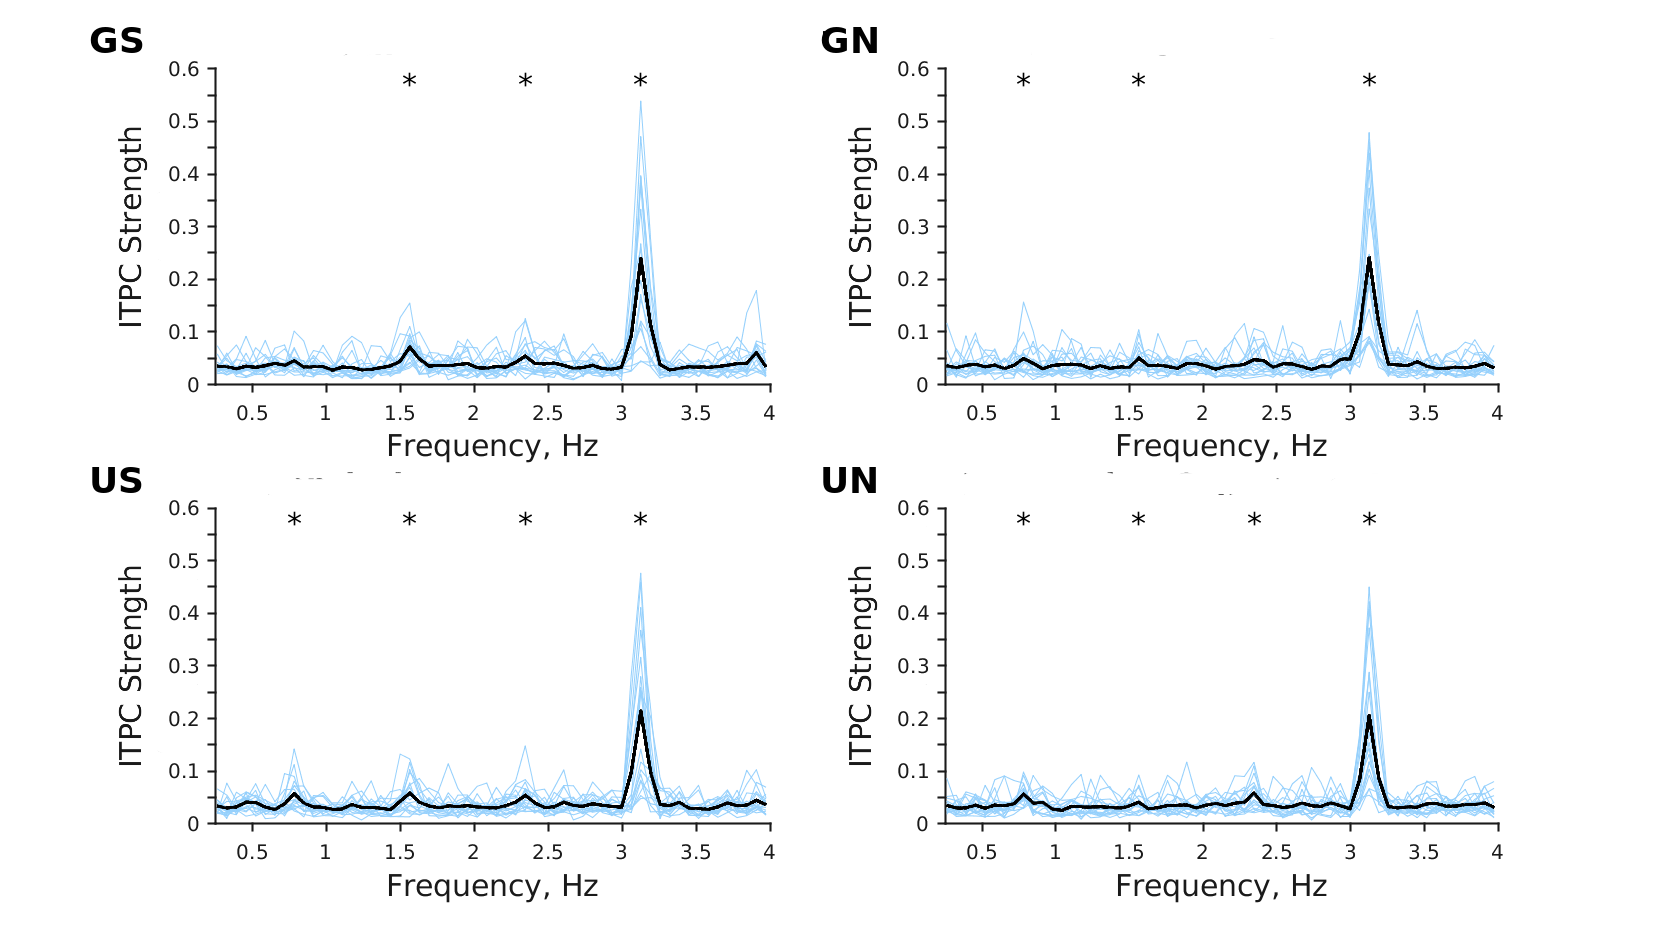
\includegraphics[width=\linewidth]{ITPC_by_condition.png}
\caption{\textbf{The spectrum of inter trial phase coherence in the
    EEG response to sentences from each of the four conditions.} These
  figures show the grand average of ITPC over all participants and
  electrodes to each of the four condition; the grand average is in
  black, the blue lines are averages over all electrodes for the 18
  individual participants. Stars represent statistical significance of
  $p<0.05$.}
\label{Fig1}
\end{figure}

We analyzed whether there were significant main effects of grammar and
meaningful semantics on the strength of the inter-trial phase
coherence at each of the three frequencies of interest in the EEG
response (1/1.28 Hz, 2/1.28 Hz and 4/1.28 Hz),
Fig.~\ref{MainEffects}. A statistically significant effect of grammar
was observed at the syllabic rate, with a greater ITPC peak for
grammatically well-formed sentences ($F=14.0673$, $n=18$ subjects,
$p=0.0016$, $\mu(\mathrm{G}) = 0.2402 \pm 0.1434$, $\mu(\mathrm{U}) =
0.2096 \pm 0.1381$; here, and elsewhere $\mu(\mathrm{C})$ is the mean of
condition C with the $\pm$ indicating the standard deviation). At the
rate of phrase presentation (2/1.28 Hz) there was a significant main
effect (Fig.~\ref{MainEffects}B) of both grammar and semantics: both
correct grammar and sensible semantics were associated with a
significantly greater peak in ITPC strength at the phrasal rate than
sentences with incorrect grammar or semantically unrelated words
(grammar: $F=14.0673$, $n=18$ subjects $p=0.0016$, $\mu(\mathrm{G})=
0.2402 \pm 0.1434$, $\mu(\mathrm{U})= 0.2096 \pm 0.1381$; semantics:
 $F=12.5283$, $n=18$ subjects, $p=0.0025$, $\mu(\mathrm{S}) = 0.0648
\pm 0.0328$, $\mu(\mathrm{N}) = 0.0459 \pm 0.0226$). No interaction
effects were observed ($p=0.7530$).

At the syllabic rate there was a significant main effect of grammar
(Fig.~\ref{MainEffects}C). The ITPC peak at the syllabic rate was
significantly greater when participants listened to grammatically
correct sentences compared to when the same participants listened to
grammatically incorrect sentences. No significant main
effect of semantics was observed (Fig.~\ref{MainEffects}C). At the
rate of sentence presentation no significant main effects on the
strength of ITPC were observed (Fig.~\ref{MainEffects}A).


%% include figure here detailing main effects results from repeated measures 2 way ANOVA.

\begin{figure}[tbp]
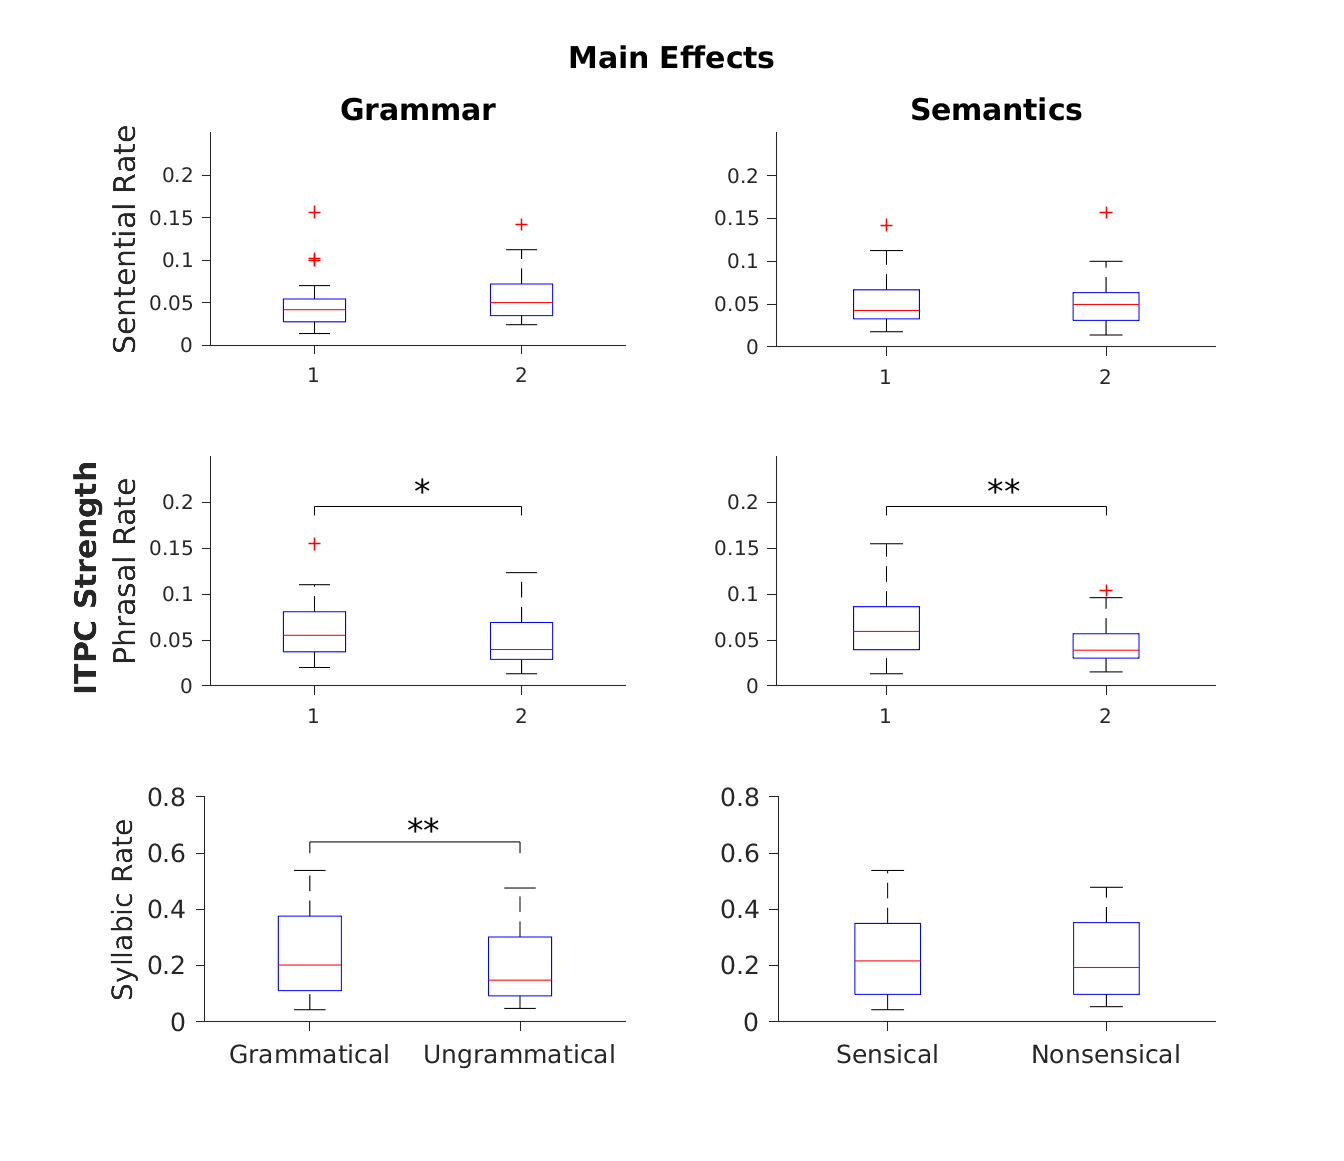
\includegraphics[width=\linewidth]{BoxPlots_main_effects.png}
\caption{\textbf{Main effects from the repeated measures 2-way ANOVA.}
  The main effects of grammar and sensible semantics on the strength
  of the ITPC at each of the three target frequencies of interest
  (1/1.28 Hz, 2/1.28 Hz and 4/1.28 Hz). A statistically significant
  effect of grammar was observed at the syllabic rate, with a greater
  ITPC peak for grammatically well-formed sentences.  A main effect of
  grammar and semantics was also observed at the phrasal rate. No interactions
  between grammar and semantics are present. 
  *: $p<0.05$, **:$p<0.005$.  }
\label{MainEffects}
\end{figure}

The ITPC response at both the sentential and syllabic rate was similar
across all of the four conditions (Figure~\ref{ITPC_peaks}A,
~\ref{ITPC_peaks}C). We next compared the strength of the ITPC at the
rate of phrase presentation between each of the four experimental
conditions (Figure ~\ref{ITPC_peaks}B). The strength of the ITPC at
the phrasal rate is significantly greater in response to grammatically
well-formed, semantically sensible sentences in condition GS
($\mu(\mathrm{GS}) = 0.0712 +/- 0.0309$) compared to both condition GN
($p = 0.0328$, $\mu(\mathrm{GN}) = 0.0507 \pm 0.0242$) and condition
UN ($p = 0.0015$, $\mu(\mathrm{UN}) = 0.0411 \pm 0.0205$). No other
comparisons were significant.

\begin{figure}[tbp]
%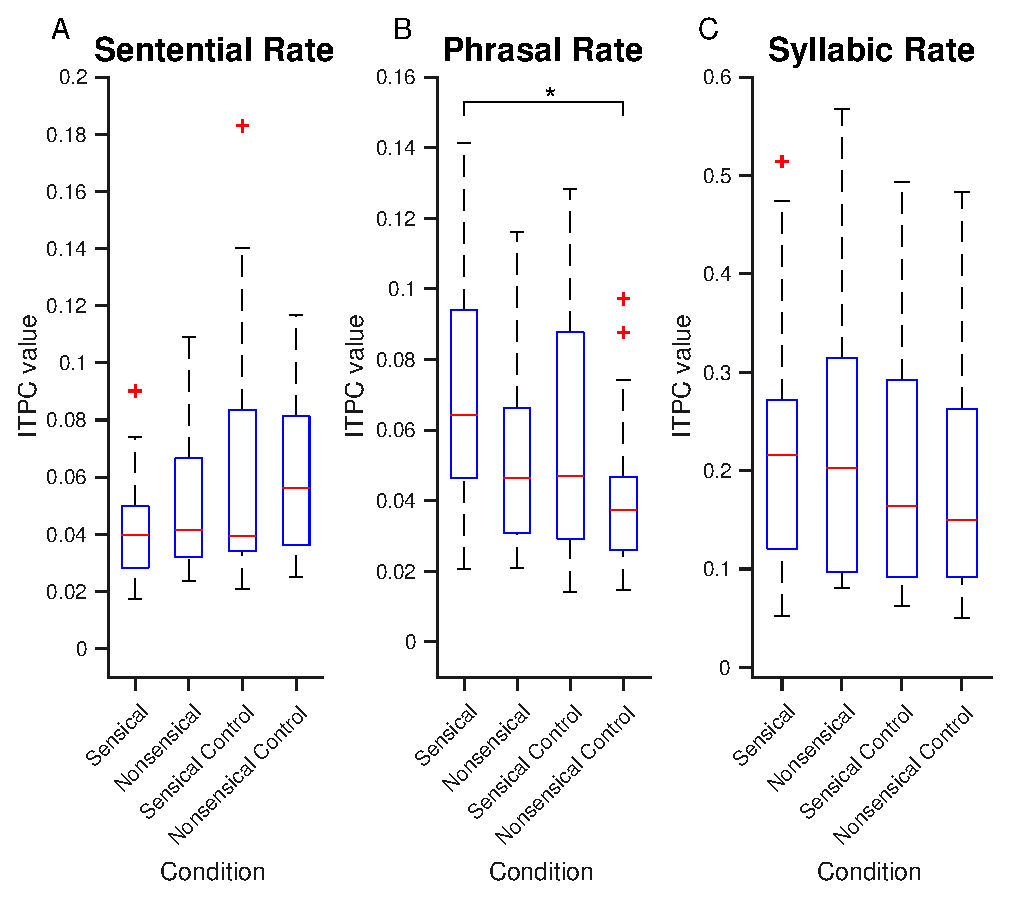
\includegraphics[width=\linewidth]{Figure3.eps}
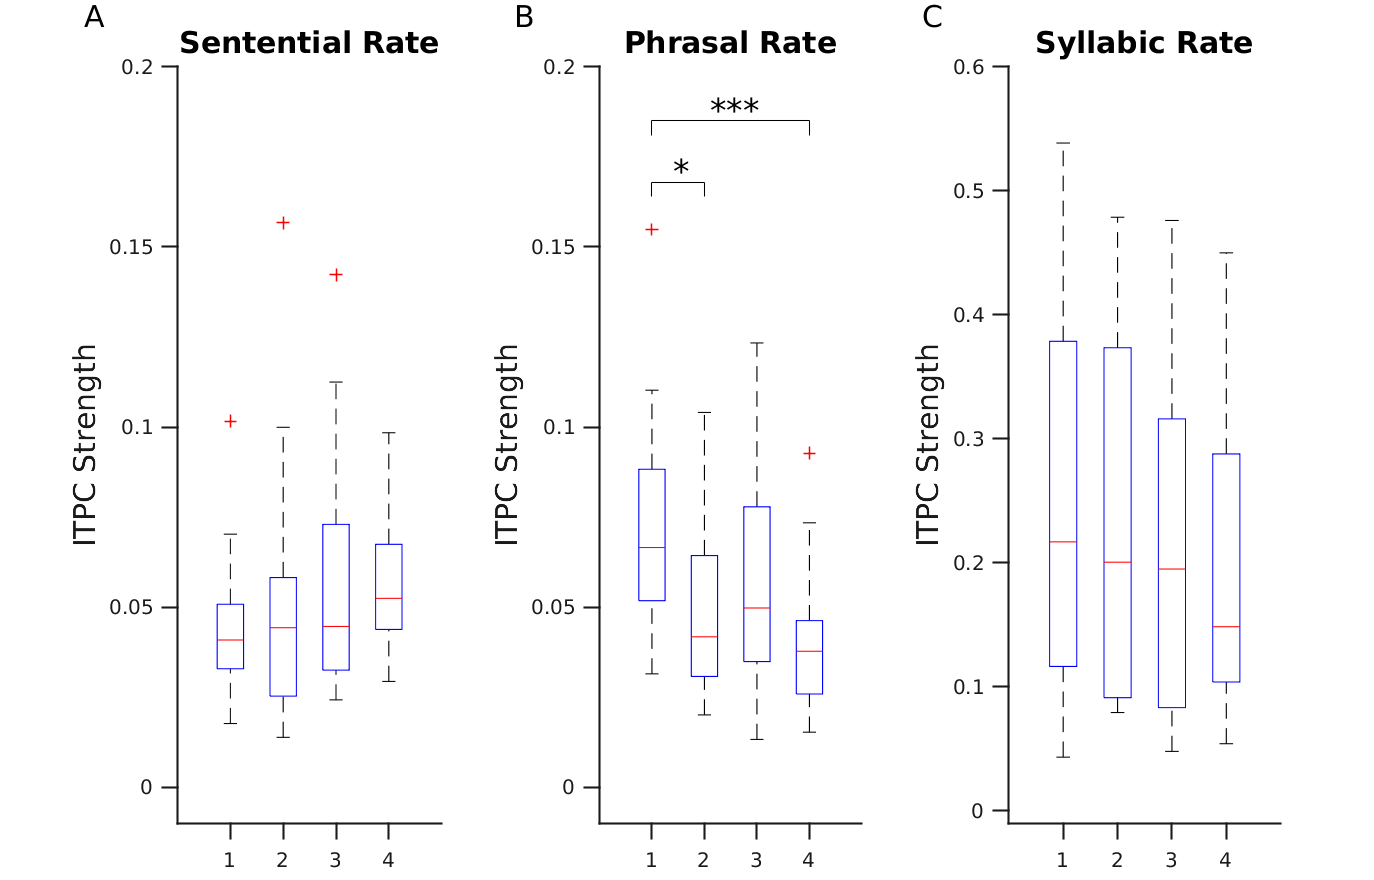
\includegraphics[width=\linewidth]{ITPC_peaks.png}
\caption{\textbf{Comparing ITPC values at frequencies of interest
    across conditions} Graphs showing average ITPC values at the
  sentential, phrasal and syllabic rates (\textbf{(A-C)}; 1/1.28 Hz,
  1/0.64 Hz, 1/0.32 Hz, respectively) for each of the four conditions
  tested. These are numbered along the $x$-axis as 1 - GS, 2 - GN, 3 -
  US and 4 - UN.  On the box plots the the central red line indicates
  the median ITPC value for each condition at each of the target
  frequencies \textbf{(A-C)}, the bottom and top edges of the box
  indicate the 25th and 75th percentiles of the ITPC values,
  respectively. The whiskers extend to the most extreme data points
  not considered outliers, and the outliers are plotted individually
  using the '+' symbol.  At the phrasal rate the GS condition is
  significantly higher than GN and UN. *:$p<0.05$, **:$p<0.005$,
  ***:$p<0.0005$. }
\label{ITPC_peaks}
\end{figure}

No effect of time was observed in the present study. The ITPC graphs
were similar when comparing trials that occurred at the beginning of
each experiment compared with trials that occurred later, and when
comparing the responses to sentences that were presented during the
first half of each trial with the last half of each trial. In cases
where conditions US and UN were presented to participants before
either conditions GS or GN, the peak in ITPC at the 1/1.28 Hz rate was
still evident. Therefore, the peak observed in ITPC at the sentential
rate to presentation in the ungrammatical conditions were not the
result of the expectancy of four word sentences given by the prior
presentation of sentences from the grammatical conditions.

\section*{Discussion}

We used EEG to record cortical activity in response to sentences
composed of four single-syllable words that can combine to form a noun
phrase and a verb phrase. We found that neural responses become
phase-locked to the frequencies at which syllables, phrases and
sentences are presented. This replicates the MEG and EEG studies
reported in \cite{DingEtAl2015,DingEtAl2017}. In this study we find:
\begin{itemize}
\item a peak in the ITPC value at the sentential rate even if the stimuli are not well formed sentences;
\item both grammar and semantics effect the ITPC value at the phrase rate.  
\end{itemize}
It is notable that the sentence peak (1/1.28 Hz) does not differ
across conditions, but the phrase peak (2/1.28 Hz) is significantly
different between conditions one and four and one and two. This
indicates that the phrase peak cannot be explained as a resonance of
the sentence peak.


In experimental conditions \textbf{US} and \textbf{UN}, the four-word
sentences are ungrammatical and do not consitute well-formed
sentences. The only information that occurs at the sentential rate is
therefore the repetition of words that share a common syntactic
category at the same position across sentences. For example, a verb is
repeated every four words. The peak at the sentential rate appears,
therefore, be driven by the repetition of an adjective, verb, subject
and object at the first, second, third and fourth position in every
sentence presented.

Our results combine to suggest that semantic information plays a
considerable role during natural language comprehension. The presence
of an ITPC peak at the sentential rate, even in the absence of
syntactic information or semantically related words, is indicative of
statistical processing at the word-level driven by syntactic category
information.

This is supported by the fact that the occurrence of a particular word
does not usually allow for good prediction of the words that follow
it. As \cite{Pulvermuller2002}, states, it is likely that the regularities
governing word sequencies likely operate over lexical category. This
means that the presentation of a pronoun for example can predict, with
high probability, the later occurance of a compliment verb. For this
to be possible abstraction over word category is necessary. Our
results are inline with this theory.

In \cite{ChristiansenChater2016} it is argued that the key to
understanding the relationship between language and language
processing is to consider how serial processing of linguistic input
can occur despite the relatively small capacity of short term memory
and the long-range global dependencies present in language. Central to
their description is \lq{}chunk-and-pass\rq{}, the aggregating and
translating of sequential elements. This chunk-and-pass operation
occurs at multiple levels going from phonemes to words, words to
phrases, phrases to clauses and so on; the key idea is that in
linguistic processing, whenever possible, sets of sequential units are
translated into a unit with a more abstract representation. For the
\lq{}chunked\rq{} representation to be more compressed than the units
it replaces, there should be some dependency between these
units.

The findings presented here are consistient with this chunk-and-pass
description of language processing; in the GS condition the sentences
fall into natural chunks based on the syntax of the sentence, these
chunks are readily represented abstractly because the constituent
words for meaningful phrases and the process of chunking is aided by
the semantic regularity of the sentences. For the UN condition all these
elements are absent and the lack of a phrase peak in the ITPC perhaps
indicates that little chunking occurs at the phrase level. From the
perspective of chunk-and-pass it is perhaps surprising that there is a
phrasal peak for condition three, composed of re-ordered sensical
sentences; these sentences should lack any phrasal structure, however,
it would appear that the semantic relatedness of some proximal words
is sufficient for some chunking to occur at the phrase rate. This
suggests that semantics plays an important role in the comprehension of
spoken sentences.

In a recent intracranial recording study reported in
\cite{FedorenkoEtAl2016} neural activity was recorded from the surface
of the brain while participants read sentences. Sentences consisted of
eight words and were either of a sensical form whereby word meaning
and grammar were correct, a \lq{}Jabberwocky\rq{} form where sentences were
well structured grammatically but had no overall sensible meaning, or
a word list form with no syntactic structure. A fourth condition was
non-word lists. Gamma-power was used to index neural activity, and was
found to increase monotonically over the course of an entire sentence
as it was read by the participant. This increase was absent in
non-word lists. In response to Jabberwocky sentences and word-lists
with the same word length the monotonic increase in gamma-power was
still evident, but to a lesser degree than when participants read
sensible sentences. As in the experiment reported here, this seems to
indicate that the increase in gamma power observed in response to
sensible sentences could not be explained by either word meaning or
syntax alone and that sentence understanding is a compositional
process. The construction of linguistic meaning may rely on both
semantic and syntactic interpretation.

It is possible that syntax and semantics can overlap to a certain
degree. \cite{Pulvermuller2002} suggests that the brain's responses to
words reflect both word semantics and lexical status;
\cite{KempsonEtAl2016} go further and suggest that syntax relies on
the incremental building of semantic representations. The experiment
reported here suggests that both correct syntactic and predictable
semantics need to occur together to generate a full brain response
during sentence comprehension. 

Hierarchical processing accounts suggest that the brain makes use of
learned grammatical knowledge to make sense of sentences, whereas in
sequential processing the brain makes use of prediction and principles
of serial order. It is likely that these two descriptions are not
mutually exclusive, but describe different aspects of the mechanisms
that work together to facilitate the rapid comprehension of sentences
during normal language processing. The current study aims to test
whether sequential accounts of language processing, relying on
word-level statistics, are more likely to explain experimental data
than hierarchical phrase-structure building operations. 

In this study sentences could come from one of four conditions. In condition one, sentences
were syntactically correct and made semantic sense. Condition two
shared the same grammatical structure as one, but were meaningless
semantically. In conditions three and four, the syntactic structure
was reordered so that the grammar was incorrect but adjectives, verbs
and nouns were all repeated at the same place within each sentence. In
condition three sentences were made up from reordered words in
sentences from condition one, whereas the sentences in condition four
contained reordered words from condition two. We found evidence in
support of sequential processing strategies. The peak in ITPC at the
sentential rate remained when grammar was incorrect but syntactic
category information was repeated at the sentential rate. The phrasal
peak in this condition was absent, and greatest when both semantic and
syntactic information were meaningful. We therefore argue in favour of
the sequential nature of language processing during simple sentence
comprehension.


\bibliographystyle{clin}         
\bibliography{Sentences}

\end{document}

